\documentclass[11pt]{scrartcl}
\usepackage[T1]{fontenc}
\usepackage[a4paper, left=3cm, right=2cm, top=2cm, bottom=2cm]{geometry}
\usepackage[activate]{pdfcprot}
\usepackage[ngerman]{babel}
\usepackage[parfill]{parskip}
\usepackage[utf8]{inputenc}
\usepackage{kurier}
\usepackage{amsmath}
\usepackage{amssymb}
\usepackage{xcolor}
\usepackage{epstopdf}
\usepackage{txfonts}
\usepackage{fancyhdr}
\usepackage{graphicx}
\usepackage{prettyref}
\usepackage{hyperref}
\usepackage{eurosym}
\usepackage{setspace}
\usepackage{units}
\usepackage{eso-pic,graphicx}
\usepackage{icomma}
\usepackage{pdfpages}

\definecolor{darkblue}{rgb}{0,0,.5}
\hypersetup{pdftex=true, colorlinks=true, breaklinks=false, linkcolor=black, menucolor=black, pagecolor=black, urlcolor=darkblue}



\setlength{\columnsep}{2cm}


\newcommand{\arcsinh}{\mathrm{arcsinh}}
\newcommand{\asinh}{\mathrm{arcsinh}}
\newcommand{\ergebnis}{\textcolor{red}{\mathrm{Ergebnis}}}
\newcommand{\fehlt}{\textcolor{red}{Hier fehlen noch Inhalte.}}
\newcommand{\betanotice}{\textcolor{red}{Diese Aufgaben sind noch nicht in der Übung kontrolliert worden. Es sind lediglich meine Überlegungen und Lösungsansätze zu den Aufgaben. Es können Fehler enthalten sein!!! Das Dokument wird fortwährend aktualisiert und erst wenn das \textcolor{black}{beta} aus dem Dateinamen verschwindet ist es endgültig.}}
\newcommand{\half}{\frac{1}{2}}
\renewcommand{\d}{\, \mathrm d}
\newcommand{\punkte}{\textcolor{white}{xxxxx}}
\newcommand{\p}{\, \partial}
\newcommand{\dd}[1]{\item[#1] \hfill \\}

\renewcommand{\familydefault}{\sfdefault}
\renewcommand\thesection{}
\renewcommand\thesubsection{}
\renewcommand\thesubsubsection{}


\newcommand{\themodul}{Optische Technologie}
\newcommand{\thetutor}{Prof. Rateike}
\newcommand{\theuebung}{Übung 2}

\pagestyle{fancy}
\fancyhead[L]{\footnotesize{C. Hansen}}
\chead{\thepage}
\rhead{}
\lfoot{}
\cfoot{}
\rfoot{}

\title{\themodul{}, \theuebung{}, \thetutor}


\author{Christoph Hansen \\ {\small \href{mailto:chris@university-material.de}{chris@university-material.de}} }

\date{}


\begin{document}

\maketitle

Dieser Text ist unter dieser \href{http://creativecommons.org/licenses/by-nc-sa/4.0/}{Creative Commons} Lizenz veröffentlicht.

\textcolor{red}{Ich erhebe keinen Anspruch auf Vollständigkeit oder Richtigkeit. Falls ihr Fehler findet oder etwas fehlt, dann meldet euch bitte über den Emailkontakt.}

\tableofcontents


\newpage



\section{Aufgabe 1}


\subsection*{a)}

Für den Lichtstrom gilt allgemein:

\begin{align*}
\phi &= K(\lambda) \cdot V(\lambda) \cdot \phi_e \qquad \text{mit} \qquad K = K_m = \unit[683]{lm/W}
\intertext{Da nur \unit[2]{\%} am Auge ankommen rechen wir dies runter:}
\phi_e &= 500 \cdot 0,02 = \unit[10]{W} \\
\Rightarrow \phi &= K_m \cdot V(500nm) \cdot 10 = 683 \cdot 0,35 \cdot 10 = \unit[2390,5]{lm}
\end{align*}


\subsection*{b)}

\begin{align*}
I_e &= \frac{\d \phi_e}{\d \Omega} = \frac{\phi_e}{4 \pi} = \frac{500}{4 \pi} = \unit[39,78]{W/sr} \\
I &= \frac{\phi}{4 \pi} = \frac{2390,5}{4 \pi} = \unit[190,22]{lm/sr}
\end{align*}


\subsection*{c)}

\begin{align*}
M_e &= \frac{\phi_e}{A} = \frac{500}{50 \cdot 10^{-4}} = \unit[10^5]{W/m^2}
\end{align*}


\subsection*{d)}

Wir betrachten einfach eine Kugel mit dem Radius $r = \unit[2]{m}$.

\begin{align*}
E_e &= \frac{\d \phi_e}{\d A} = \frac{500}{4 \pi r^2} = \frac{500}{4 \pi \cdot 2^2} = \unit[9,95]{W/m^2} \\
E &= 683 \cdot 0,35 \cdot 9,95 = \unit[2378]{lm/m^2}
\end{align*}


\subsection*{e)}

\begin{align*}
\phi_e &= 9,95 \cdot A_{Loch} = 9,95 \cdot \pi \cdot 0,05^2 = \unit[0,0195]{w} \\
\phi &= K \cdot V(\lambda) \cdot \phi_e = 683 \cdot 0,35 \cdot 0,0195 = \unit[4,66]{lm}
\end{align*}


\section{Aufgabe 2}

\subsection*{a)}

\begin{align*}
V(441) &\approx 0,05 \qquad q_e = \unit[10]{mW} \\
V(633) &\approx 0,3 \qquad q_e = \unit[4]{mW} 
\intertext{Damit ergeben sich relative Helligkeiten von:}
\phi_{441} &= 683 \cdot 0,05 \cdot 10^{-2} = \unit[0,34]{lm} \\
\phi_{633} &= 683 \cdot 0,3 \cdot 4 \cdot 10^{-3} = \unit[0,82]{lm}
\end{align*}


\subsection*{b)}

\begin{align*}
V(488) &\approx 0,25 \\
V(543) &\approx 0,8 
\intertext{Nun soll gelten, das die Helligkeiten gleich sein sollen. Dazu setzen wir gleich:}
\phi(488) &= \phi(543) \\
\Leftrightarrow 683 \cdot 0,25 \cdot \phi_{Ar} &= 683 \cdot 0,8 \cdot 0,5 \cdot 10^{-3} \\
\Leftrightarrow \phi_{Ar} &= \frac{0,8 \cdot 0,5 \cdot 10^{-3}}{0,25} = \unit[1,6]{mW}
\end{align*}


\section{Aufgabe 3}

Zuerst eine Zeichnung zur Erläuterung:

\begin{figure}[h]
	\centering
	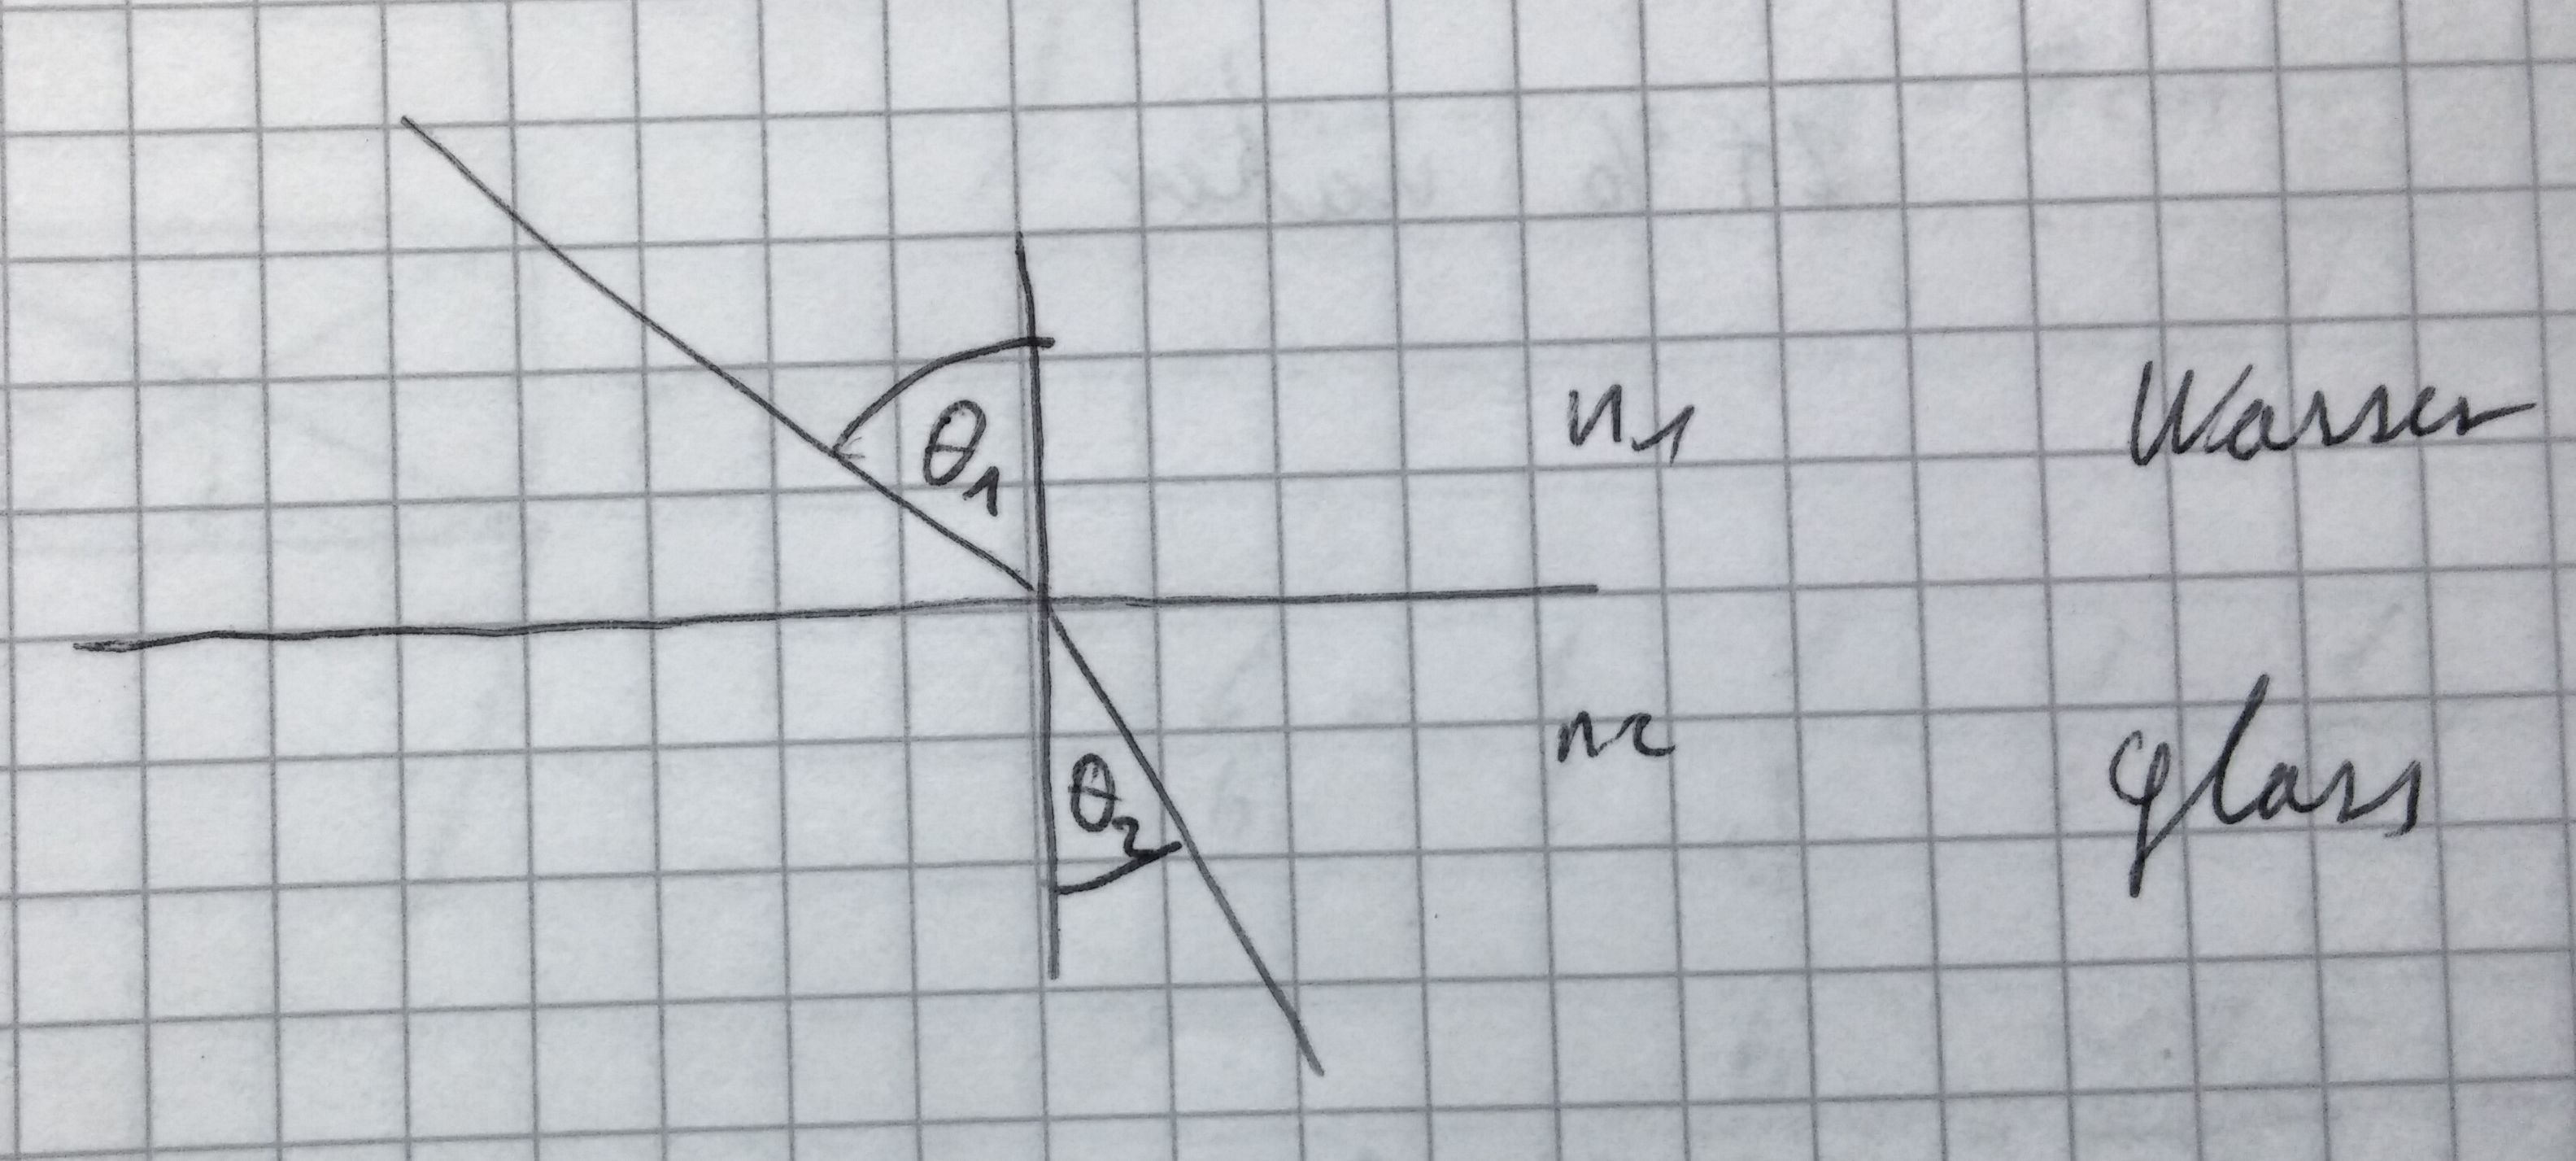
\includegraphics[scale=0.1]{A3_1.jpg}
\end{figure}


Wir wissen das die Beleuchtungsstärke so definiert $\frac{lm}{m^2}$, wir versuchen dies nun anders darzustellen:

\begin{align*}
\frac{lm}{m^2} &= \frac{lm}{sr} \cdot \frac{sr}{m^2} \\
\intertext{Wir bestimmen nun den letzten Teil des Terms:}
\Delta \Omega &\approx \frac{A}{r^2} = \frac{1}{3^2} = \unit[\frac{1}{9}]{sr/m^2}
\intertext{Jetzt können wir einfach umstellen und ausrechnen:}
E &= \frac{1}{9} \cdot I \\
\Leftrightarrow I &= 9 \cdot E = 9 \cdot 100 = \unit[900]{lm/sr}
\end{align*} 

\subsection*{b)}

Wir berechnen hier den Abschwächungsfaktor, der einen Meter neben dem Punkt $P$ anzuwenden ist:

\begin{figure}[h]
	\centering
	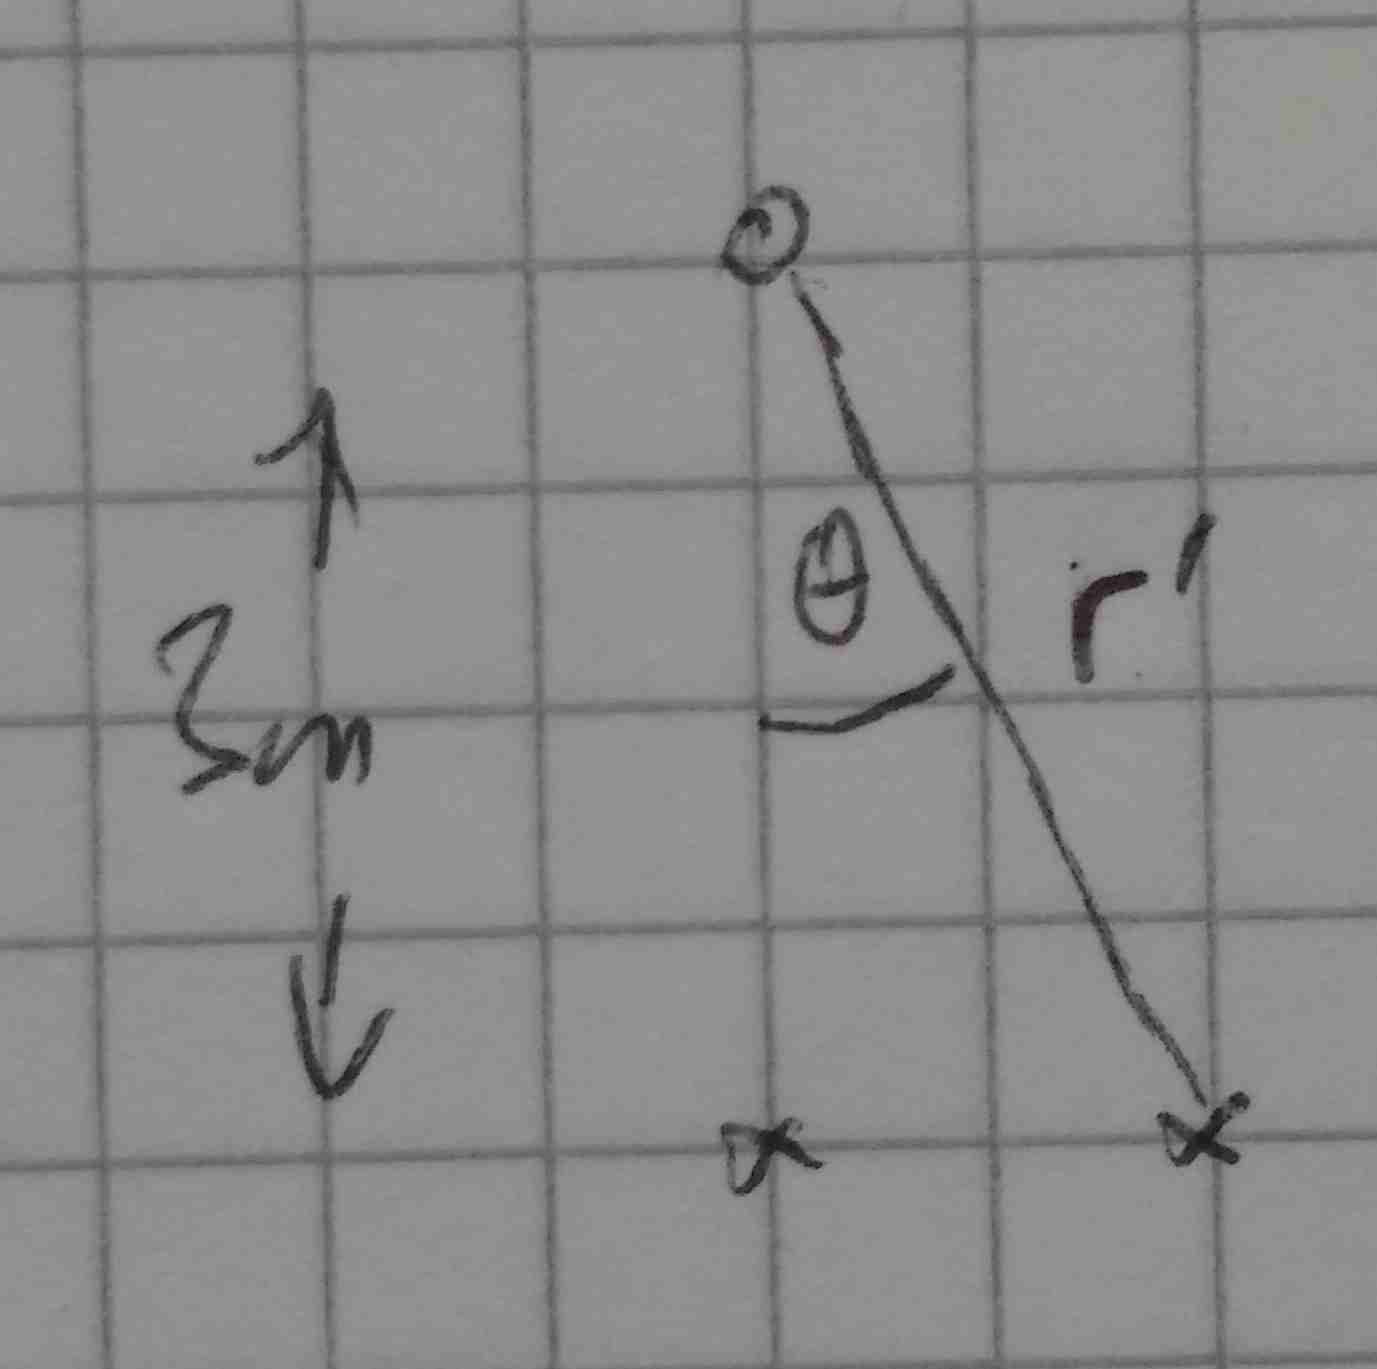
\includegraphics[scale=0.1]{A3_2.jpg}
\end{figure}


\begin{align*}
r' &= \sqrt{3^2 + 1^2} = \sqrt{10} \\
\theta &= \arctan \left( \frac{1}{3} \right) = 18,434
\intertext{Der Abscwächungsfaktor ist dann:}
x &= \frac{r^2}{r'^2} \cdot \cos(\theta) = \frac{9}{10} \cdot \cos(18,434) = 0,853 \\
\Rightarrow E' &= 100 \cdot x = 85,3
\end{align*}






















\end{document}